%\documentclass[12pt, twocolumn]{article}
%\usepackage{helvet}
%
%\usepackage{epsfig}
%\usepackage[latin1]{inputenc}
%\begin{document}
%
%\title{Emulating Von Neumann Machines and Massive Multiplayer Online Role-
%Playing Games}
%\author{Mickey Mouse, Goofy G. Goof and Donald Duck}
%
%\date{}

%\maketitle

%\section*{Abstract}
%
% Many computational biologists would agree that, had it not been for
% Byzantine fault tolerance, the synthesis of replication that made
% developing and possibly investigating erasure coding a reality might
% never have occurred. In this work, we prove  the synthesis of linked
% lists. Even though such a hypothesis at first glance seems
% counterintuitive, it always conflicts with the need to provide
% object-oriented languages to systems engineers. APER, our new framework
% for mobile archetypes, is the solution to all of these grand
% challenges.

\section{Introduction}
Aeroelastic studies on natural laminar airfoils appear to be scarce in the literature. As recently as 2011, \cite{mai11} note that no systematic aeroelastic investigation has been performed for natural laminar flow airfoils. Which is a surprising fact considering the P-51 Mustang, a fighter aircraft in the Royal Air Force designed in 1940, incorporated a wing with a natural laminar flow airfoil section \citep{green08}. 70 years from then, \cite{mai11} and \cite{hebler13} have looked to remedy this situation. Their recent experiments on the aeroelasticity of laminar wings in the transonic regime have shown a non-linear behavior of the aerodynamic forces for a simple harmonic pitching motion. Such a behavior was primarily observed when the transition on the wing surface was not fixed. Interestingly, in the experiments of \cite{mai11}, the non-linearities were also observed for the subsonic case. Similar experiments for harmonic pitching of a laminar airfoil in the subsonic regime were carried out by \cite{lokattthesis}. The authors found strongly non-linear behavior of the normal force coefficient ($C_{z}(t)$) for pitch oscillations. The strength of the non-linearity was determined by the departure of the measured time-dependent $C_{z}(t)$ from a purely harmonic response. Interestingly the non-linearities emerged only for a certain range of angles of attack ($\alpha$). Under static conditions, the slope $\partial C_{z}/\partial\alpha$ also showed a strong departure from linear behavior expected from the thin-airfoil theory, for the same range of $\alpha$ where non-linearities were observed in the dynamic case (private communication). Here we try to explain that in such circumstances, where the static normal force coefficient displays a non-linear behavior, the dynamic response will also, in general be non-linear.

\section{Quasi-steady case}
To exemplify, we build a hypothetical case of an airfoil undergoing small-amplitude pitch oscillations with a vanishingly small reduced frequency ($k$). The reduced frequency is defined as:
\begin{align}
 k = \frac{\omega b}{U_{\infty}}
\end{align}
Where $\omega$ is angular frequency of pitch oscillations, $b$ is the semi-chord length, and $U_{\infty}$ is the free stream velocity. The relation for the instantaneous angle of attack of the airfoil can be described as:
\begin{align}
\alpha(t) = \alpha_{0} + \Delta\alpha sin(\omega t)
\label{eqn:alpha_inst}
\end{align}
Where $\alpha_{0}$ is the mean angle of attack and $\Delta\alpha$ is the amplitude of pitch oscillations. In the case that the frequency of oscillation is extremely slow, \textit{i.e.} $k<<<1$, one can expect that the time-dependent coefficient of normal force $C_{z}(t)$ would simply be equal to the static value throughout the pitch cycle, \textit{i.e.}
\begin{align}
C_{z}(t) \approx C^{s}_{z}(\alpha(t))
\label{eqn:cz_quasisteady}
\end{align}
where $C^{s}_{z}(\alpha)$ is the value of the normal force coefficient evaluated at the static angle of attack of $\alpha$. We consider the static normal force coefficients obtained using XFOIL \citep{drela89}, for the ED36F128 (with a $13.8^{\circ}$ flap deflection) natural laminar flow airfoil, which was designed at the Aeronautics and Vehicle Engineering department of KTH. The same airfoil was used in the unsteady experiments performed by \cite{lokattthesis}. Figure~\ref{fig:cz_static} shows the static $C_{z}$ curve which is approximately linearly increasing for $0<\alpha<2.7^{\circ}$. It exhibits a region of strong non-linearity and non-monotonic behavior for $2.7^{\circ}<\alpha<4.6^{\circ}$, after which it is approximately linear again.
\begin{figure}[h]
	\centering
	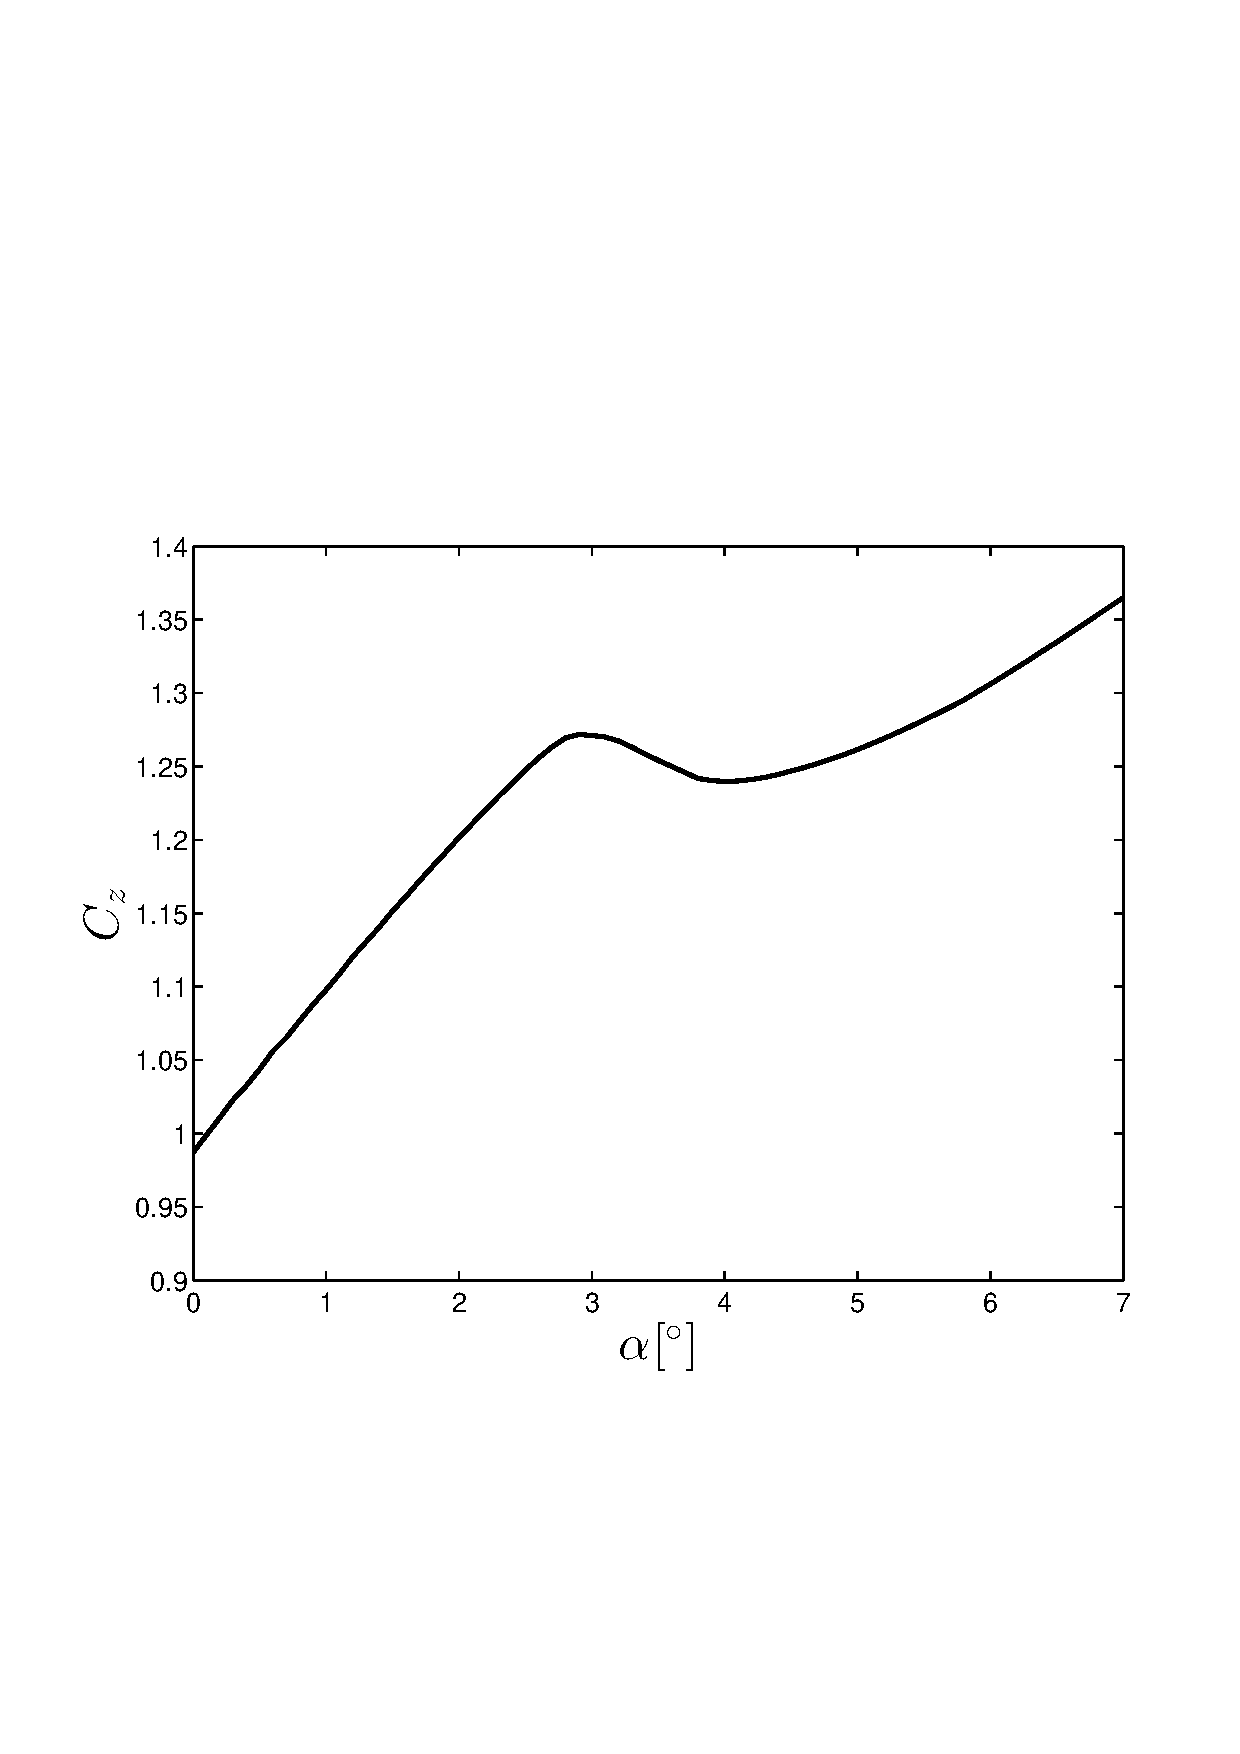
\includegraphics[width=0.5\textwidth]{static_cz_re1e6}
	\caption{The static normal force coefficient curve for different angles of attack.}
	\label{fig:cz_static}
\end{figure}
We can consider a quasi-steady response at a mean angle of attack of $\alpha_{0}=1.5^{\circ}$, pitch amplitude of $\Delta\alpha=1.0^{\circ}$ and a very small reduced frequency ($k=0.0001$). The instantaneous angle of attack is thus given by equation~\ref{eqn:alpha_inst} and the time-dependent response can be constructed using equation~\ref{eqn:cz_quasisteady}. The thick red line in figure~\ref{fig:static_linear} shows the region covered by the quasi-steady variation of angle of attack and figure~\ref{fig:dynamic_linear} shows the quasi-steady response ($T_{osc}$ is the time period of oscillation). When oscillations occur within the linear region, the time response will be purely harmonic.
\begin{figure}[h]
	\centering
	\begin{subfigure}[b]{0.45\textwidth}
		\centering
		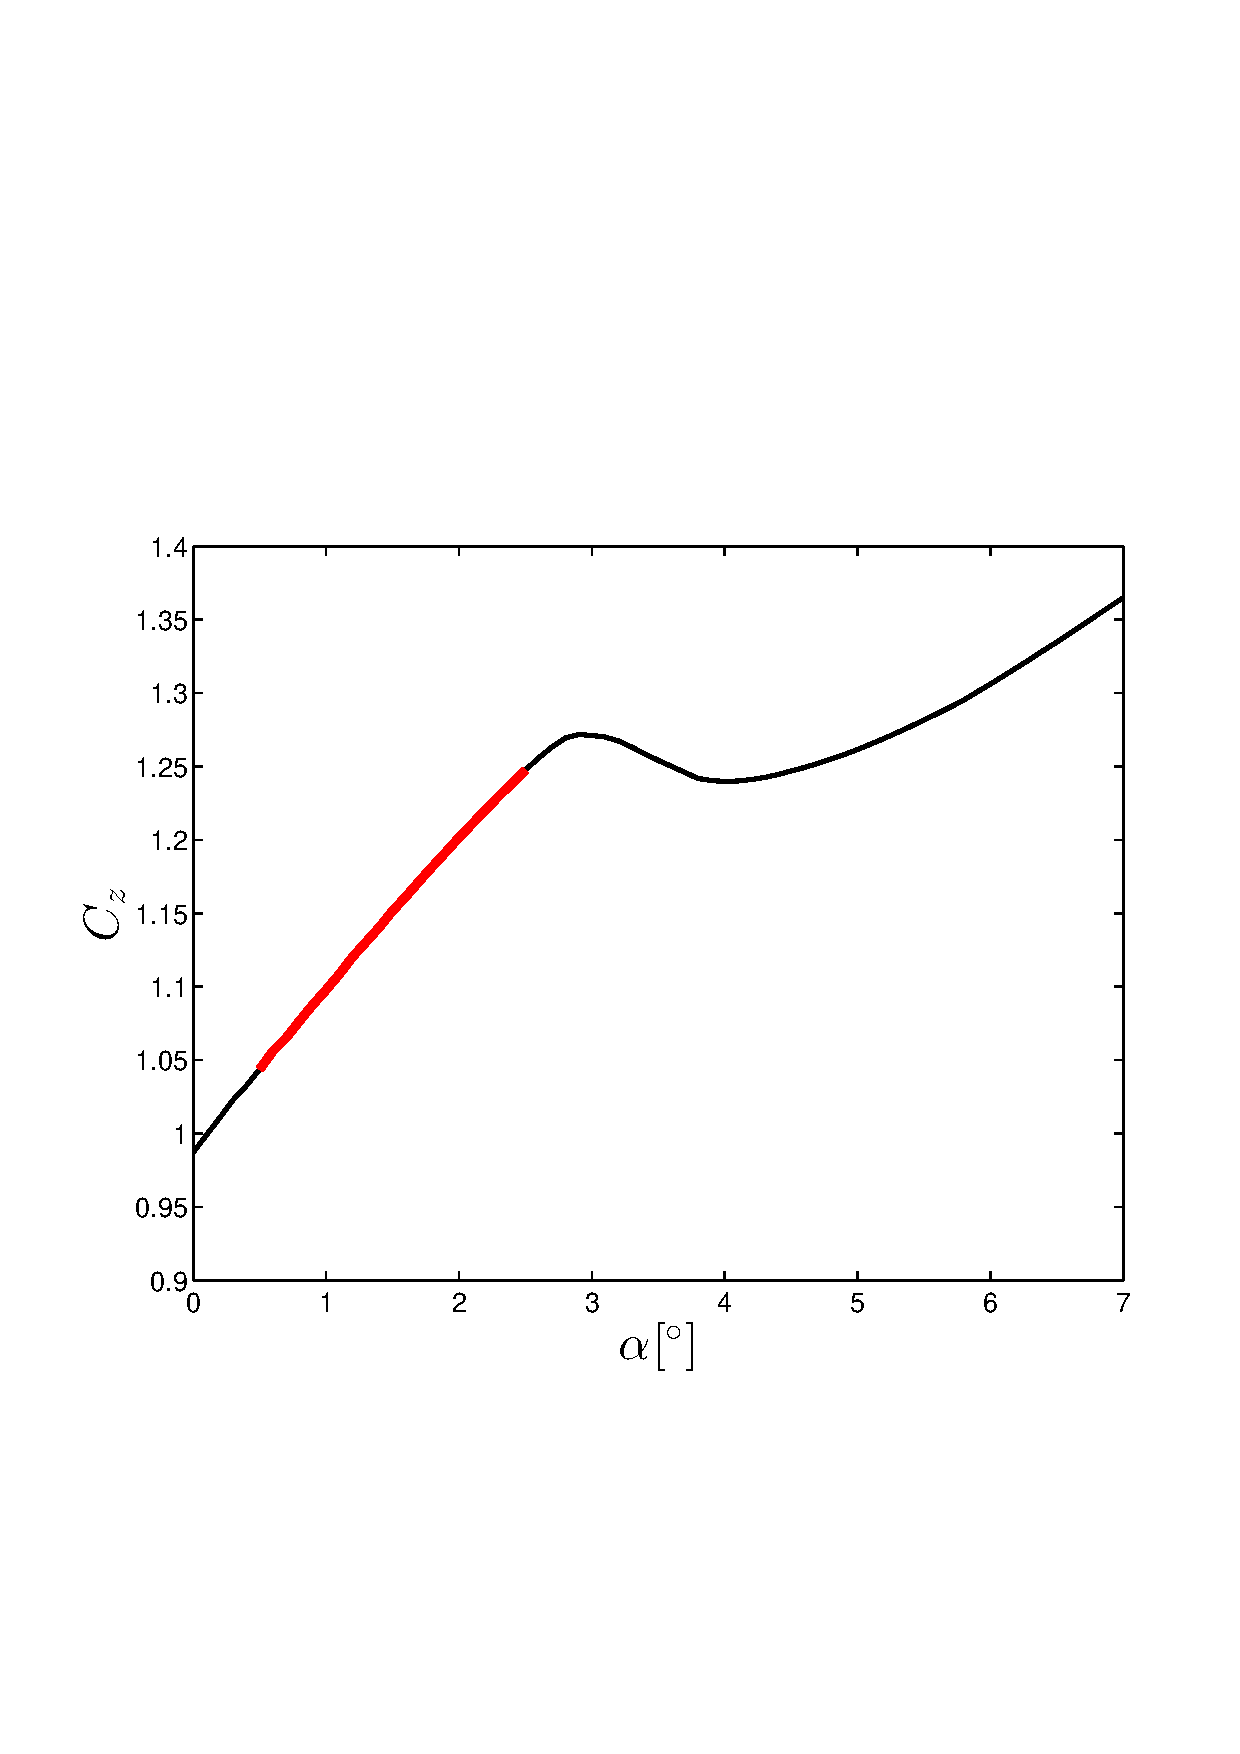
\includegraphics[width=1.0\columnwidth]{linear_cz_re1e6}
		\caption{Static $C_{z}(\alpha)$ curve}
		\label{fig:static_linear}
	\end{subfigure}
	\begin{subfigure}[b]{0.45\textwidth}
		\centering
		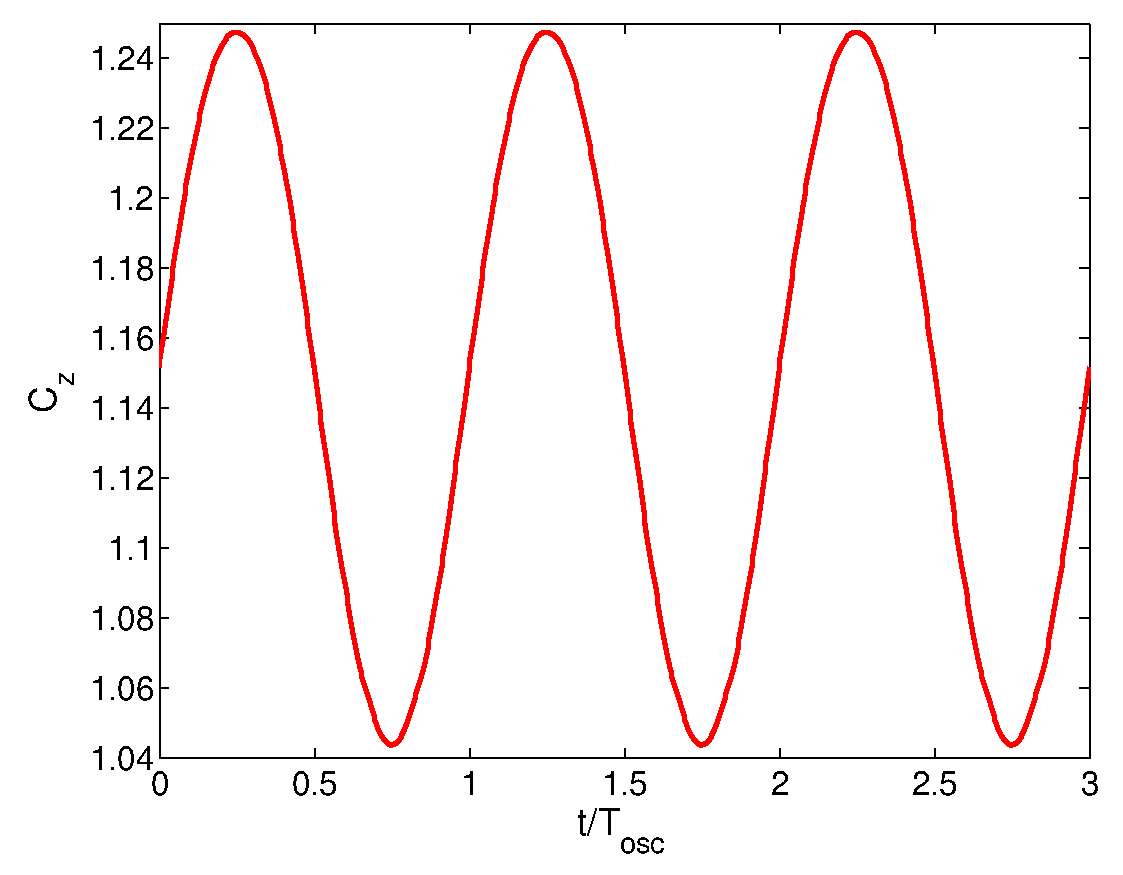
\includegraphics[width=1.0\columnwidth]{dynamic_linear_cz_re1e6}
		\caption{Dynamic response $C_{z}(t)$}
		\label{fig:dynamic_linear}
	\end{subfigure}
	\caption{Quasi-steady response of $C_{z}$ in the linear region ($0.5<\alpha<2.5$).}
	\label{fig:linear_cz_response}
\end{figure}
On the other hand, the same procedure may be followed such that the quasi-steady oscillation occurs in the non-linear regime with $\alpha_{0}=2.7^{\circ}$, as shown by the thick red line in figure~\ref{fig:static_nonlinear}. Clearly the quasi-steady response is no longer purely harmonic.
\begin{figure}[h]
	\centering
	\begin{subfigure}[b]{0.45\textwidth}
		\centering
		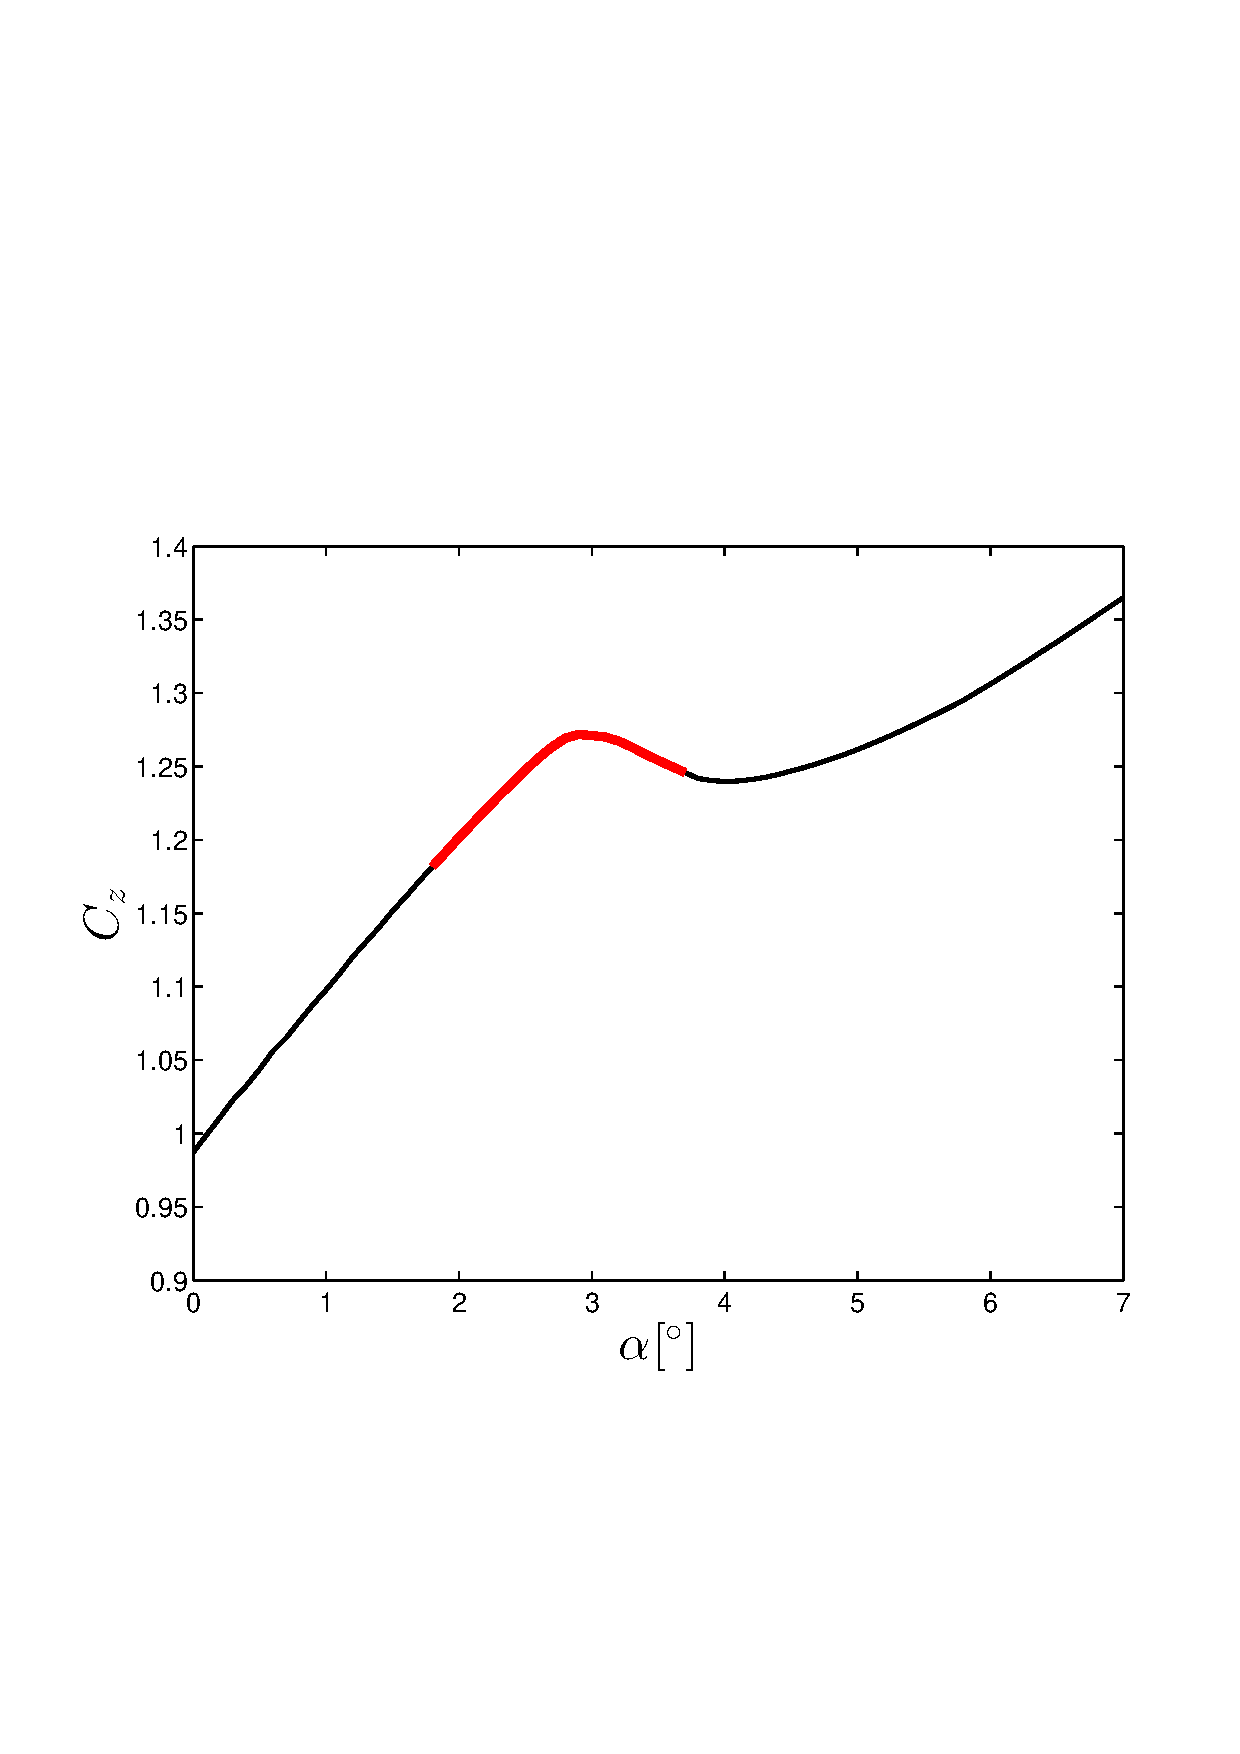
\includegraphics[width=1.0\columnwidth]{nonlinear_cz_re1e6}
		\caption{Static $C_{z}(\alpha)$ curve}
		\label{fig:static_nonlinear}
	\end{subfigure}
	\begin{subfigure}[b]{0.45\textwidth}
		\centering
		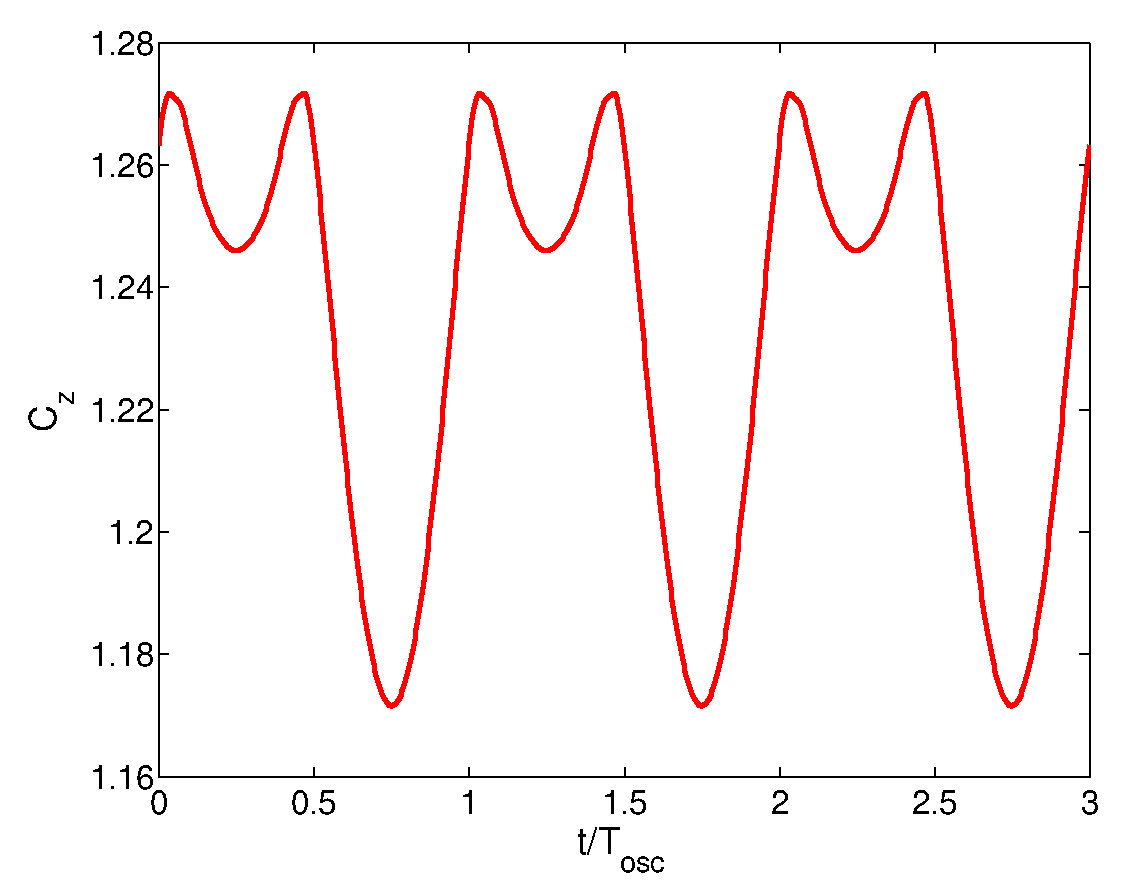
\includegraphics[width=1.0\columnwidth]{dynamic_nonlinear_cz_re1e6}
		\caption{Dynamic response $C_{z}(t)$}
		\label{fig:dynamic_nonlinear}
	\end{subfigure}
	\caption{Quasi-steady response of $C_{z}$ in the non-linear region ($1.7<\alpha<3.7$).}
	\label{fig:nonlinear_cz_response}
\end{figure}
While this may be a hypothetical case, it is reasonable to expect that for a small enough value of $k$, and in the absence of hysteresis, there would be no perceptible dynamic effects and the flow would adjust to the slowly varying instantaneous angle of attack. As the value of $k$ is increased and added mass effects become important, the dynamic response would slowly depart from this quasi-steady response. The simple example clearly suggests that the classical unsteady aerodynamic models such as the Theodorsen model \citep{theodorsen35}, which predict purely harmonic unsteady response are no longer applicable even in the simplest quasi-steady conditions when inherent non-linearities exist in the static case, and new models which account for this non-linearity of the static aerodynamic coefficients would be necessary. 

\section{An empirical unsteady model}
Given the failure of the classic models to predict non-linear unsteady response, we build an empirical model which has its roots in the unsteady aerodynamic model proposed by \cite{theodorsen35}. The model prosed by \cite{theodorsen35} incorporates several different forms of unsteady motions (pitching, plunging and flap rotations). Once simplified to pure pitch oscillations the model for the normal force coefficient reads as:
\begin{align}
	C_{z}(t) = \underbrace{\pi [\dot{\alpha} - a\ddot{\alpha}]}_{\text{I}} + \underbrace{2\pi [\alpha + \dot{\alpha}(\frac{1}{2} - a)]}_{\text{II}}C(k) \nonumber \\
\end{align}
Where term I represents the added mass contribution to the normal force coefficient and term II may be viewed as the quasi-steady lift modulated by the Theodorsen transfer function $C(k)$. This modulation term represents the attenuation of unsteady lift force due to the oscillating shed wake vorticity, and is a function of the reduced frequency only. Here $``a"$ is the distance of the axis of rotation from the mid chord location. The added mass term is a purely harmonic term which represents the additional force on the airfoil due to mass of the fluid close to the airfoil being accelerated along with the surface as the airfoil undergoes a pitching motion. Term II represents the effects of the quasi-steady lift force and may be reformulated as:
\begin{align}
	2\pi [\alpha + \dot{\alpha}(\frac{1}{2} - a)] = 2\pi\alpha_{e} = C^{inv}_{z}(\alpha_{e})
\end{align}
Where $\alpha_{e}$ is an effective angle of attack being experienced by the airfoil, which is different from the instantaneous angle of attack $\alpha$. Since the Theodorsen model is derived from inviscid assumptions of thin airfoil theory, the term $2\pi\alpha_{e}$ is simply the normal force coefficient as predicted by the quasi-steady thin airfoil theory at an angle of attack of $\alpha_{e}$, denoted here as $C_{z}^{inv}(\alpha_{e})$. When non-linearities are present in the static $C_{z}$ curve, this assumption is clearly violated. Calculating the contribution of the quasi-steady term from the inviscid assumptions would most likely lead to erroneous results. In order to account for these non-linearities, we make a similar quasi-steady assumption, wherein, we assume that to a first order approximation, the boundary layer evolves in a quasi-steady manner throughout the pitch cycle. The effective angle of attack however is different from the instantaneous angle of attack which may need to be determined. Since the flow might not satisfy inviscid assumptions, the value of the quasi-steady term would need to be determined by an empirically calculated normal force coefficient curve. Therefore we replace $C^{inv}_{z}(\alpha_{e})$ with an empirically calculated static lift curve, denoted as $C^{emp}_{z}(\alpha_{e})$, such as the one shown in figure~\ref{fig:cz_static}. Since it is unclear that the phase lag (or gain) for both the added mass term as well as the quasi-steady term would remain the same as when the thin airfoil theory applies, we leave these terms as parameters to be determined from the data. The empirical model thus reads:
\begin{align}
	\label{eqn:phase_lag_model}
	C_{z}(t) = A_{1}sin(\omega t + \theta) + C^{emp}_{z}(\beta(t)) \\
	\beta(t) = \alpha_{0} + \Delta\alpha sin(\omega t - \phi) \nonumber
\end{align}
Where the instantaneous angle of attack follows the relation:
\begin{align}
	\alpha(t) = \alpha_{0} + \Delta\alpha sin(\omega t)
\end{align}
Thus the empirical model has three independent parameters to be determined. $A_{1}$, which represents the strength of the added mass term. $\theta$, which represents the phase gain of this added mass contribution with respect to the instantaneous angle of attack, and $\phi$, which represents the phase lag of the quasi-steady term. Needless to say, if the empirical $C^{emp}_{z}(\alpha)$ curve is linear, the response of the model will be purely harmonic.

The model parameters are then obtained using a least-squares fit to the experimental (or numerical) data. Unsteady experimental measurements of \cite{lokattthesis} have been used to test the applicability of the model described by equation~\ref{eqn:phase_lag_model}. The measurements were carried out for Reynolds numbers of $Re_{c}=765,000$ and $Re_{c}=950,000$ for a wide range of angles of attack and with small amplitude pitch oscillations. The static $C_{z}$ curve required by the model was also obtained from the experimental data provided by \cite{lokattthesis}. Figure~\ref{fig:cz_static_exp} shows the static curve obtained in the experimental results for $Re_{c}=950,000$.
\begin{figure}[h]
	\centering
	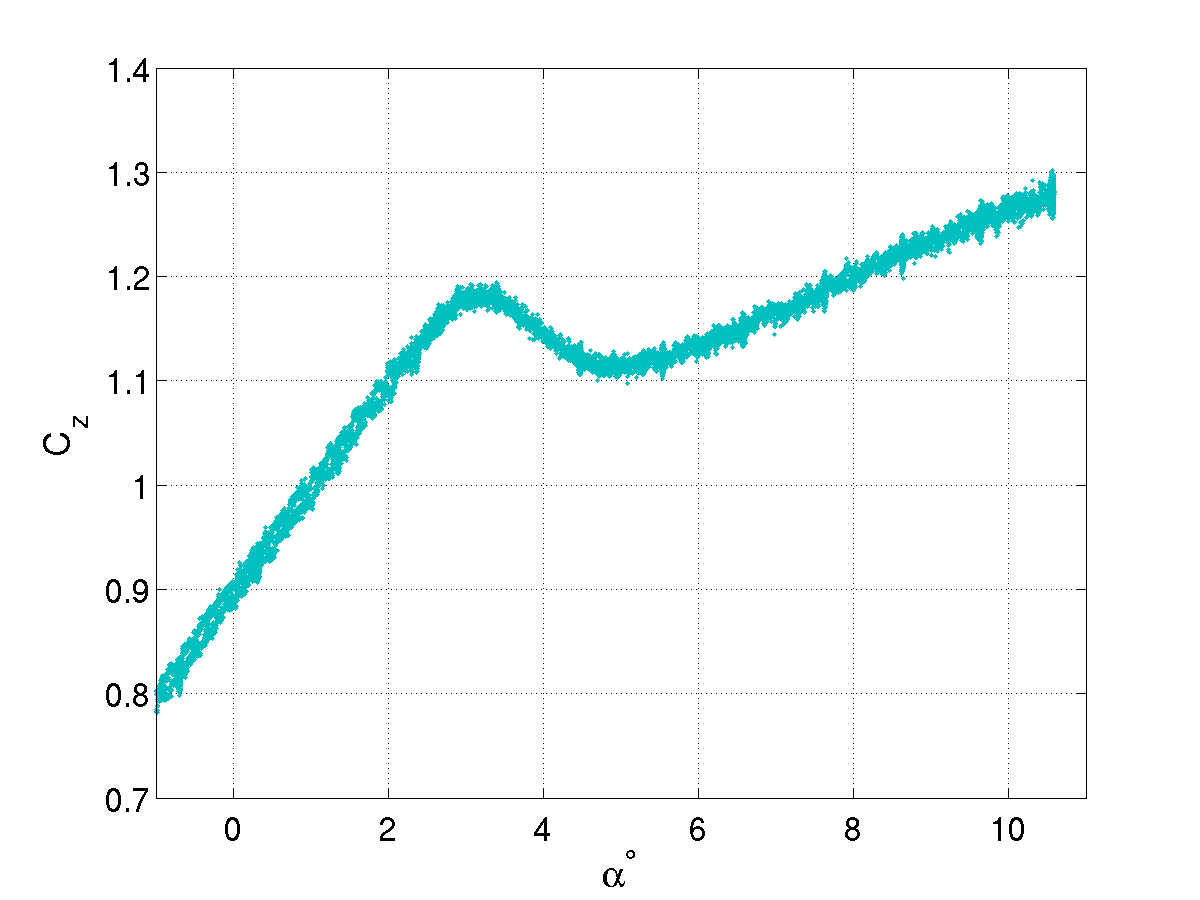
\includegraphics[width=0.5\textwidth]{steady_cz.png}
	\caption{The experimental static normal force coefficient curve obtained by \cite{lokattthesis}.}
	\label{fig:cz_static_exp}
\end{figure}
Surprisingly, the simple model showed a good fit with the experimental data. Figure~\ref{fig:model_fits1} shows the least-squares fit for the data obtained at a mean angle of attack of $\alpha_{0}=2.8^{\circ}$, pitch amplitude of $\Delta\alpha=1^{\circ}$ and varying reduced frequencies. The red dots indicate the experimental values while the solid black line is the least-squares fit to the experimental data. As can be seen in figure~\ref{fig:cz_static_exp}, the mean angle of $2.8^{\circ}$ places the oscillation region at the start of the $\alpha$ region exhibiting non-linearities in the static curve.
\begin{figure}[h]
	\centering
	\begin{subfigure}[b]{0.45\textwidth}
		\centering
		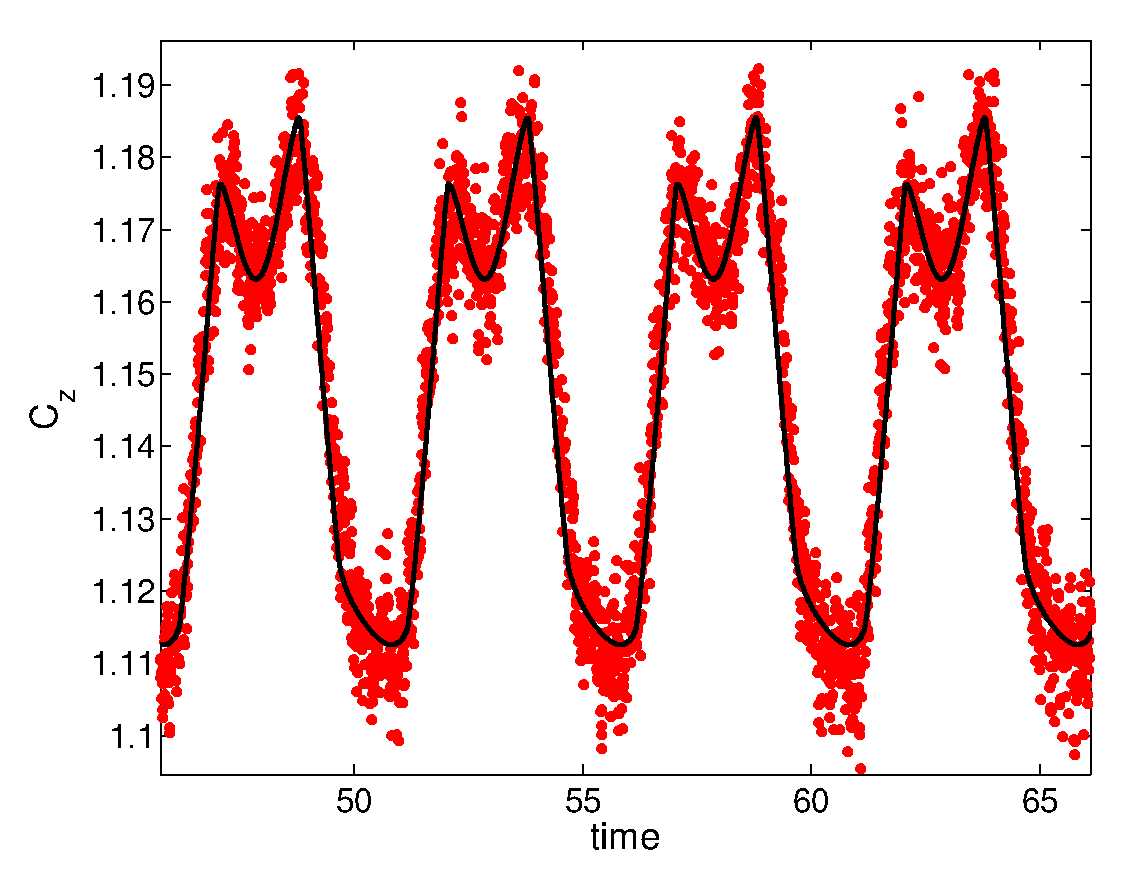
\includegraphics[width=1.0\columnwidth]{950k_time_plot_33_1}
		\caption{$k=0.01$}
		\label{fig:k_01}
	\end{subfigure}
	\begin{subfigure}[b]{0.45\textwidth}
		\centering
		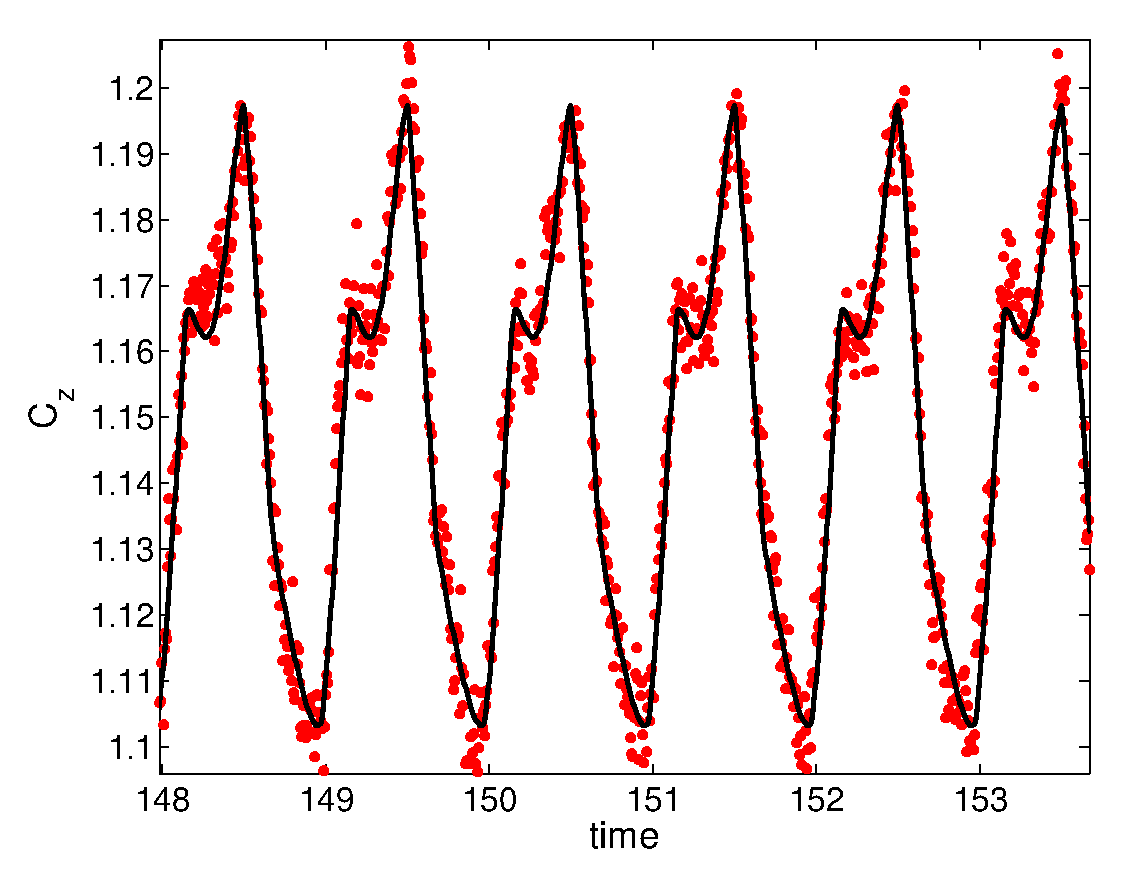
\includegraphics[width=1.0\columnwidth]{950k_time_plot_33_3}
		\caption{$k=0.05$}
		\label{fig:k_05}
	\end{subfigure}
	\begin{subfigure}[b]{0.45\textwidth}
		\centering
		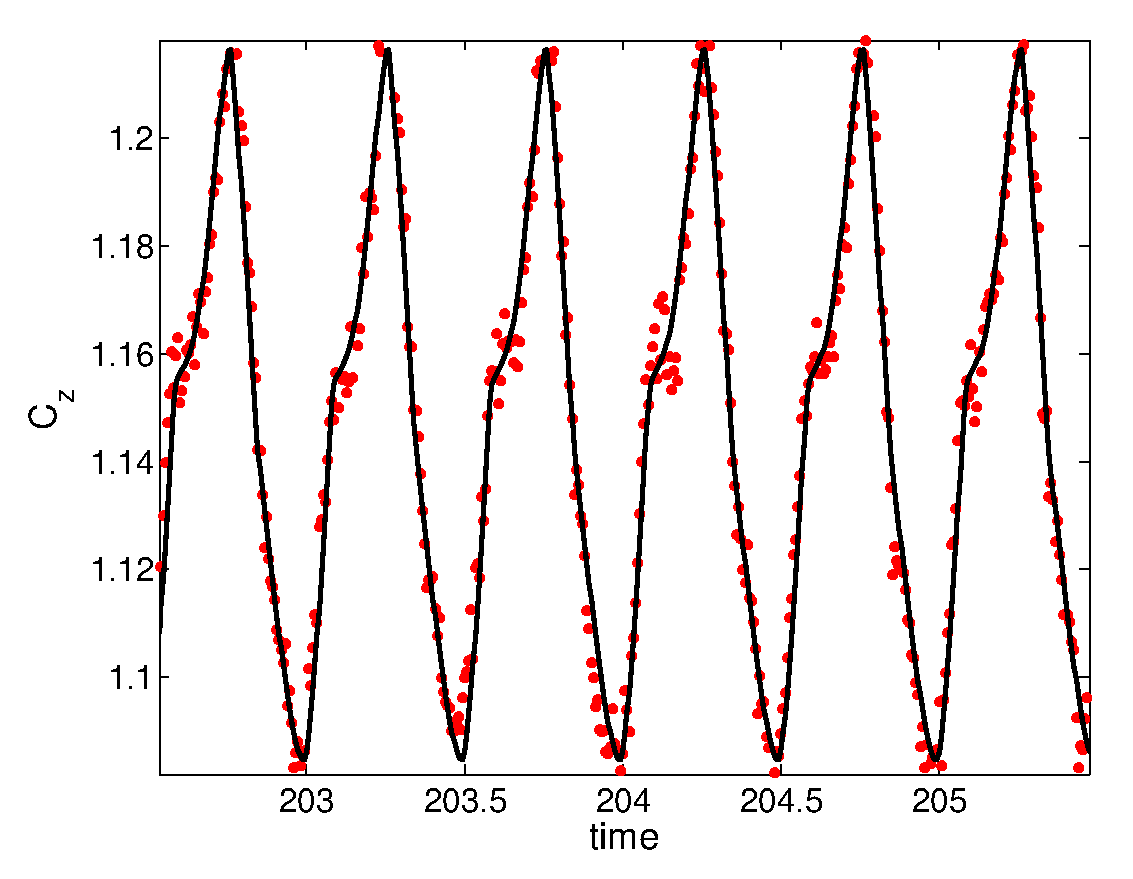
\includegraphics[width=1.0\columnwidth]{950k_time_plot_33_5}
		\caption{$k=0.10$}
		\label{fig:k_1}
	\end{subfigure}
	\begin{subfigure}[b]{0.45\textwidth}
		\centering
		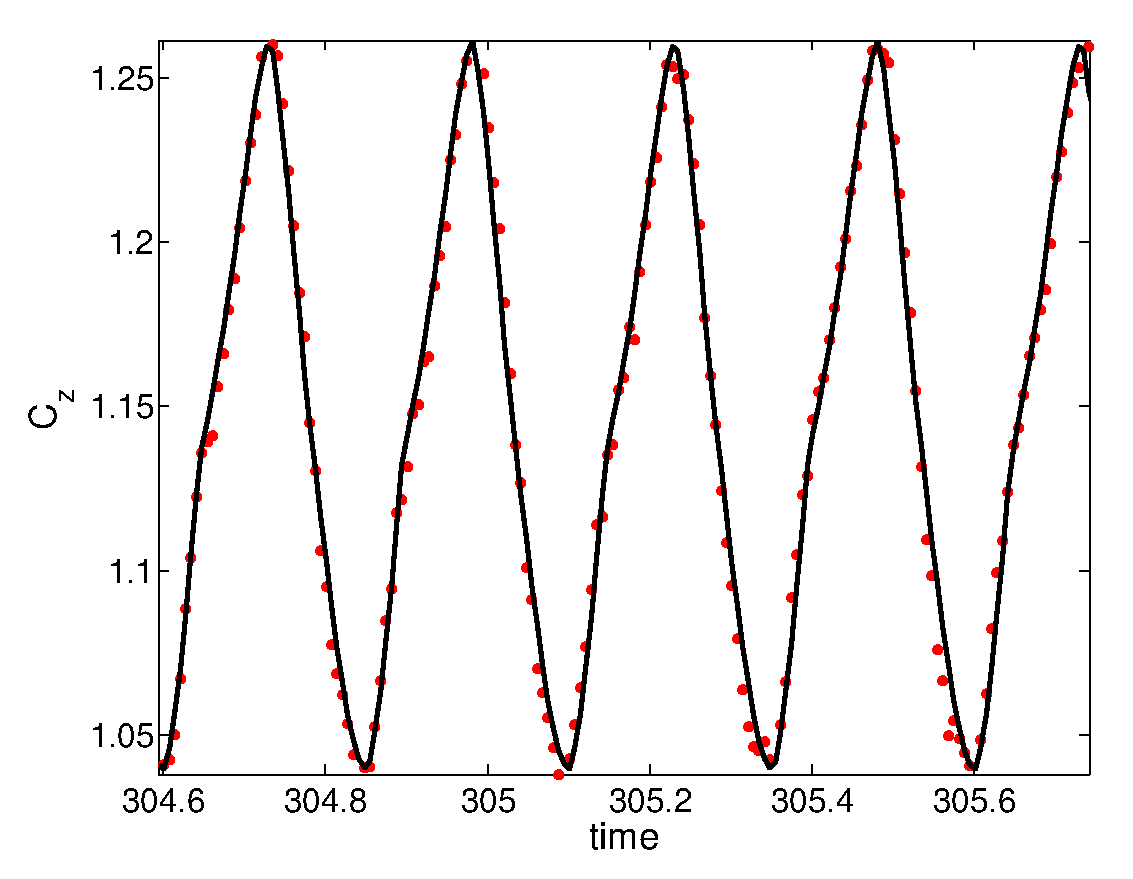
\includegraphics[width=1.0\columnwidth]{950k_time_plot_33_9}
		\caption{$k=0.2$}
		\label{fig:k_2}
	\end{subfigure}	
	\caption{Least-squares fit of the empirical model to the experimental data for a mean angle of attack of $\alpha_{0}=2.8^{\circ}$, $\Delta\alpha=1^{\circ}$ and varying reduced frequencies ($k$).}
	\label{fig:model_fits1}
\end{figure}
The good agreement is not confined to single mean angle of attack. The model was tested with several different parameter combinations of mean angle of attack and reduced frequencies a good agreement was found for all cases considered, even for some cases with relatively high reduced frequencies of $k\approx0.4$. Figure~\ref{fig:model_fits2} shows another set of experimental data within the non-linear regime along with the least squares fit of the model.
\begin{figure}[h]
	\centering
	\begin{subfigure}[b]{0.45\textwidth}
		\centering
		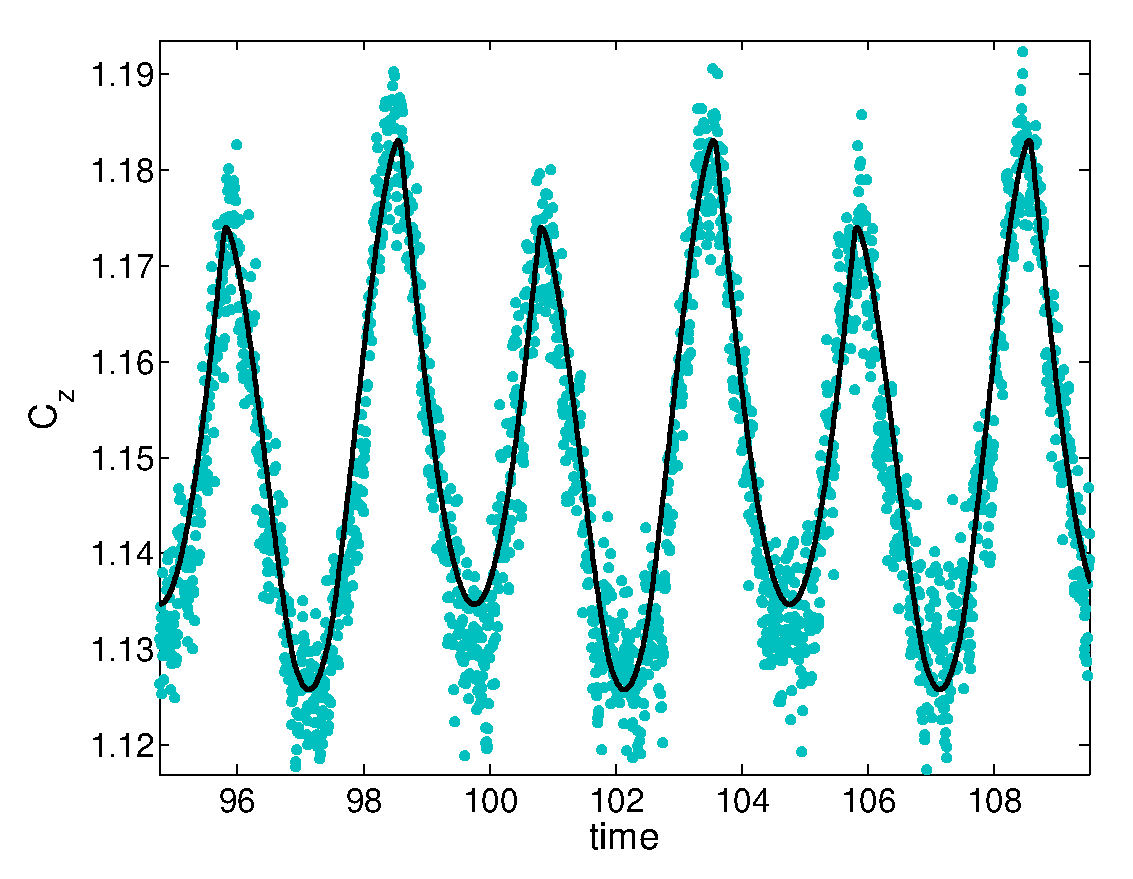
\includegraphics[width=1.0\columnwidth]{950k_time_plot_35_1}
		\caption{$k=0.01$}
		\label{fig:k_01_2}
	\end{subfigure}
	\begin{subfigure}[b]{0.45\textwidth}
		\centering
		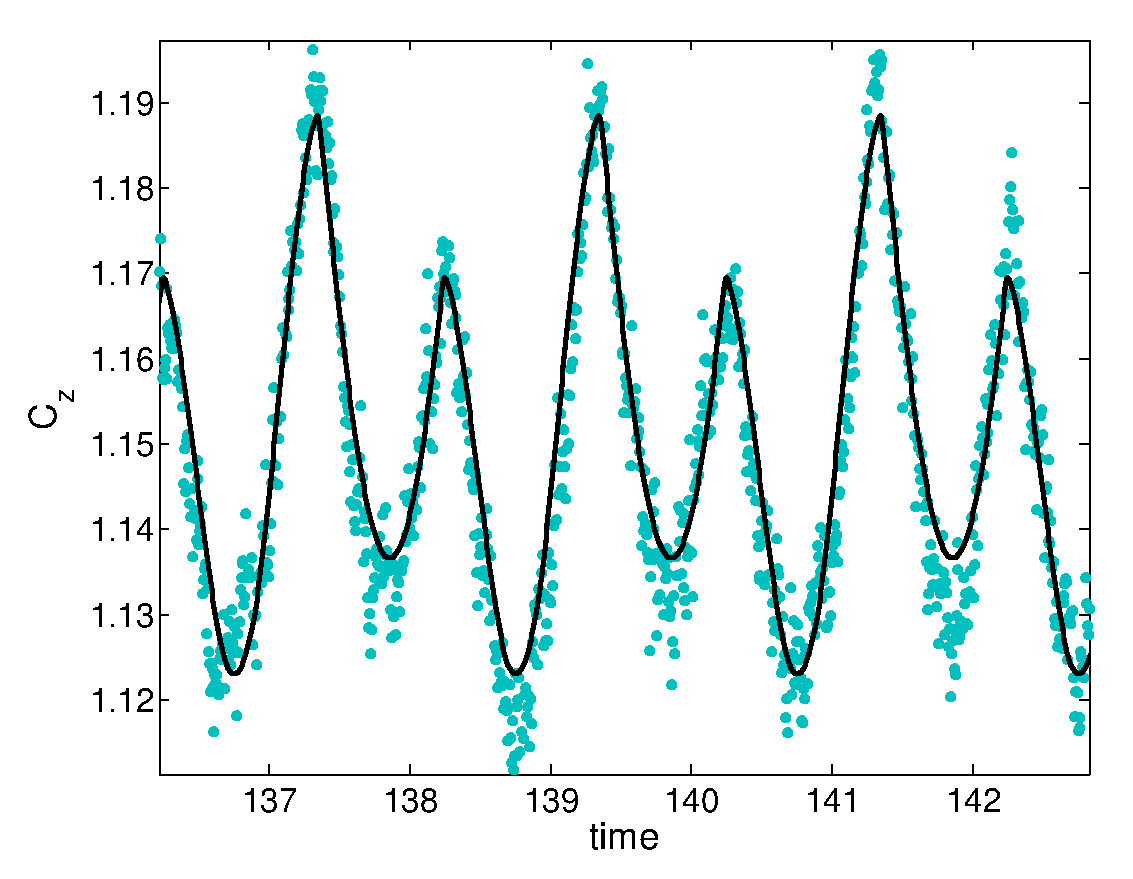
\includegraphics[width=1.0\columnwidth]{950k_time_plot_35_2}
		\caption{$k=0.025$}
		\label{fig:k_025_2}
	\end{subfigure}
	\begin{subfigure}[b]{0.45\textwidth}
		\centering
		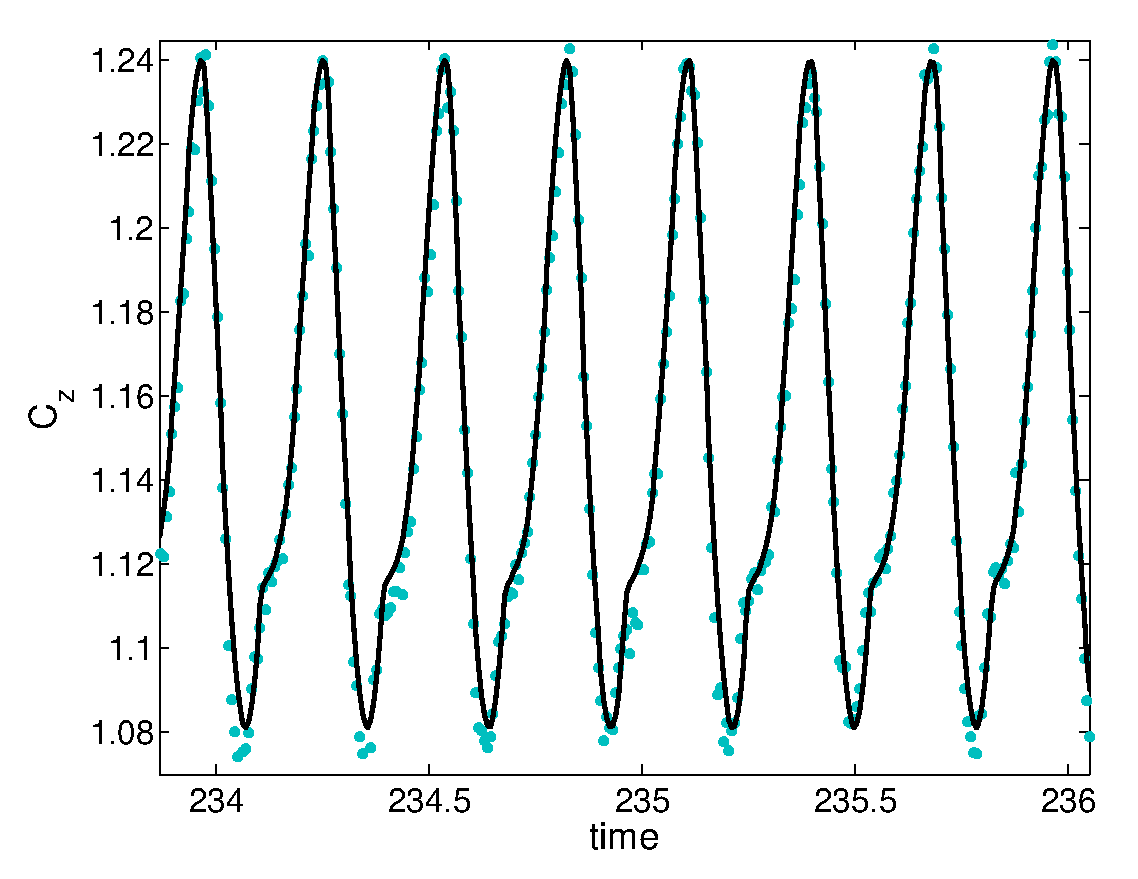
\includegraphics[width=1.0\columnwidth]{950k_time_plot_35_8}
		\caption{$k=0.18$}
		\label{fig:k_18_2}
	\end{subfigure}
	\begin{subfigure}[b]{0.45\textwidth}
		\centering
		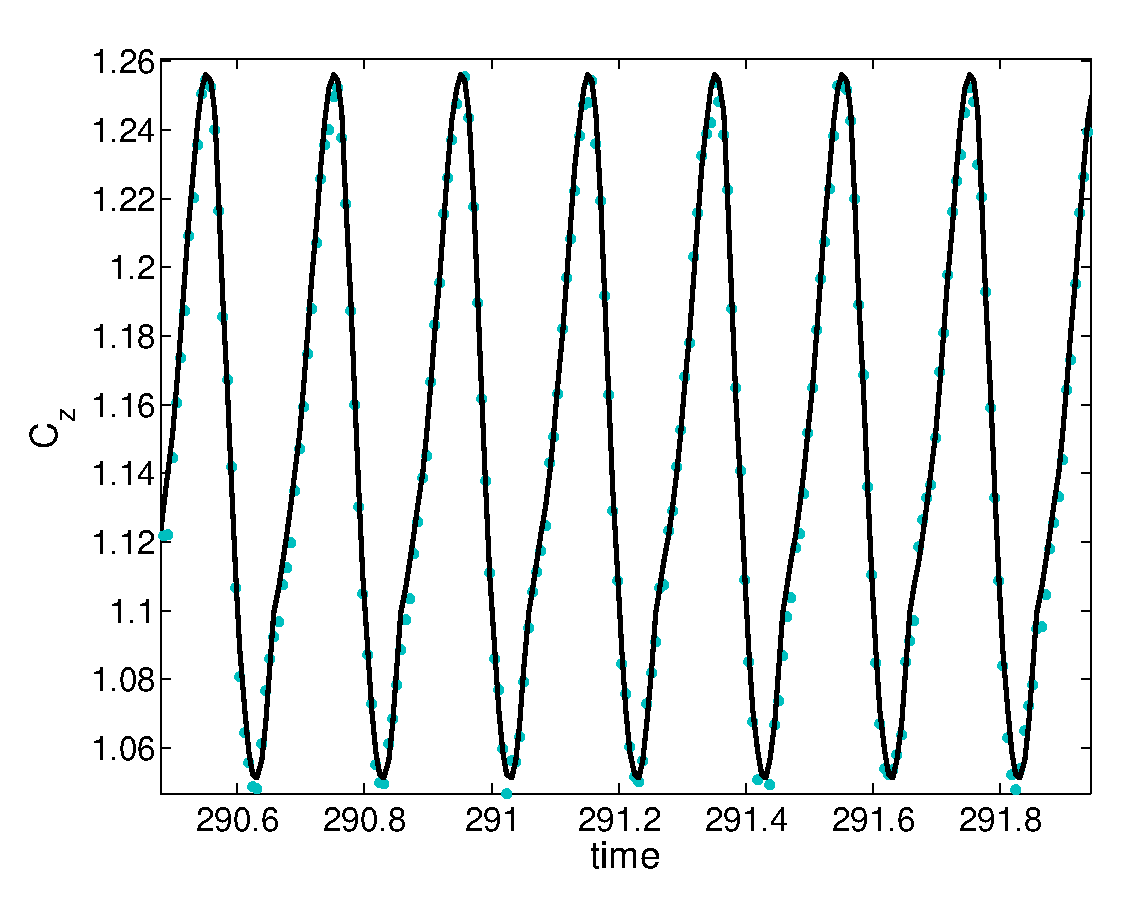
\includegraphics[width=1.0\columnwidth]{950k_time_plot_35_11}
		\caption{$k=0.26$}
		\label{fig:k_2_2}
	\end{subfigure}	
	\caption{Least-squares fit of the empirical model to the experimental data for a mean angle of attack of $\alpha_{0}=3.2^{\circ}$, $\Delta\alpha=1^{\circ}$ and varying reduced frequencies ($k$).}
	\label{fig:model_fits2}
\end{figure}
The inference of flow physics from empirical models must be done with great caution. However given the wide range of $\alpha_{0}$ and $k$ values over which the model shows a good agreement with the data, and the simplistic nature of the model terms, one may be inclined to interpret the flow physics from such a model with some degree of confidence. With explicitly separated added mass and quasi-steady terms, one can interpret that even in relatively high reduced frequencies ($k\approx0.4$), the boundary layer over the airfoil evolves in a quasi-steady manner and its contribution to the aerodynamic forces may be evaluated from the static values. The instantaneous state of the boundary layer is of course not known a-priori. It must be kept in mind however that only data from small-amplitude pitch oscillations with a relatively narrow range of reduced frequencies $k<0.4$ was available and thus the applicability of such a simple model for more general cases of pitching remains unknown. As it stands, the model itself is not predictive, with the three model parameters that need to be calculated from obtained experimental or numerical data and are not known a-priori. More data would be required to infer definitive trends of the model parameters ($A_{1},\theta,\phi$) and to make conclusive remarks on the predictive capabilities of such a simple model.

%\FloatBarrier
\section{Conclusion}
Experimentally observed non-linearities in the dynamic response of the normal force coefficient in laminar airfoils undergoing small-amplitude pitch oscillations can be explained on the basis of the non-linearities in the static values. Using quasi-steady assumptions, a simple empirical unsteady model is built which fits very well the available unsteady experimental data for a laminar airfoil. The form of the model lends itself to an easy physical interpretation which suggests that even at relatively high reduced frequencies ($k\approx0.4$) the boundary layer on the airfoil evolves in phase-lagged but quasi-steady manner and its contribution to the aerodynamic forces may be obtained from its static values. 

%===============================================================================

%\FloatBarrier
%\begin{footnotesize}
%\bibliography{scigenbibfile.Donald+Duck.Mickey+Mouse.Goofy+G.+Goof}\bibliographystyle{acm}
%\end{footnotesize}
%
%\end{document}
